\documentclass[a4paper,12 pt]{article}
\usepackage[T2A]{fontenc}
\usepackage[utf8]{inputenc}
\usepackage[english, russian]{babel}
\usepackage{geometry}
\usepackage{float}
\usepackage{amsfonts}
\usepackage{array}
\newcolumntype{C}[1]{>{\centering\arraybackslash}p{#1}}
 \geometry{
 a4paper,
 top=25mm,
 }
\usepackage{amsmath, amsfonts, amssymb, amsthm, mathtools, indentfirst, float, wrapfig}
\usepackage{wrapfig}
\usepackage{graphicx}
\graphicspath{{pictures/}}
\DeclareGraphicsExtensions{.pdf,.png,.jpg}
\begin{document}
    \begin{titlepage}
    \begin{center}
        \vspace{4cm}
        \huge {\textbf{Отчет о выполнении лабораторной работы 3.2.4(5) }}
        {} \\
        \vspace{1cm}
        \Large {\textbf{Свободные и вынужденные колебания в электрическом контуре}} \\
        \Large {\textbf{}} \\
        \vspace{10cm}
        \begin{flushright}
        \begin{minipage}{.45\textwidth}
        \normalsize{\textbf{Студент:} Копытова Виктория Сергеевна}\\
        \textbf{Группа:} Б03-304\\
        \end{minipage}
        \end{flushright}   
    \end{center}
    \end{titlepage}
\newpage
 
\section{Аннотация}
\textbf{Цель работы:} исследование свободных и вынужденных колебаний в
колебательном контуре.

\textbf{В работе используются:} осциллограф АКТАКОМ ADS-6142H, гене-
ратор сигналов специальной формы АКИП-3409/4, магазин сопротивле-
ния МСР-60, магазин емкости Р5025, магазин индуктивности Р567 типа
МИСП, соединительная коробка с шунтирующей емкостью, соединитель-
ные одножильные и коаксиальные провода.
	

\section{Теоретические сведения}

\subsection{Свободные колебания}

Схема установки для исследования колебаний приведена на рисунке 1.

Колебательный контур состоит из постоянной индуктивности L с активным со-
противлением $R_L$, переменной емкости C и сопротивления R. Картина колебаний
напряжения на емкости наблюдается на экране двухканального осциллографа. Для возбуждения затухающих колебаний используется генератор сигналов специальной
формы.
\begin{figure}[H]
    \centering
    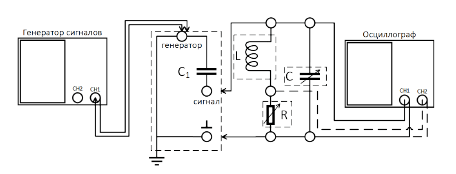
\includegraphics[scale=1]{1.png}
    \caption{Схема установки для исследования вынужденных колебаний}
    \label{fig:enter-label}
\end{figure}

Логарифмический декремент затухания
\begin{equation}
    \Theta=\frac{1}{n} \ln \frac{U_m}{U_{m+n}}    
\end{equation}

\subsection{Вынужденные колебания}

\begin{figure}[H]
    \centering
    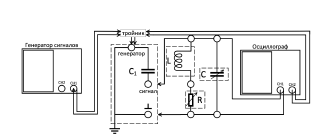
\includegraphics[scale=1.5]{2.png}
    \caption{Схема установки для исследования АЧХ и ФЧХ}
\end{figure}



\section{Ход работы}

\subsection{Активное сопротивление $R_L$ и индуктивность L}
\begin{table}[H]
    \centering
    \begin{tabular}{|c|c|c|c|c|c|}
    \hline
        $R_L$, Ом & 28.8 & 29.2 & 30.8 & 43.0 & 86.0 \\
    \hline
        L, мГн & 100.0 & 99.98 & 99.97 & 100.6 & 103.0 \\
    \hline
        $\nu$, Гц & 50 & 500 & 1500 & 5000 & 10000 \\
    \hline
    \end{tabular}
    \caption{Активное сопротивление $R_L$ и индуктивность L}
\end{table}

\begin{figure}[H]
    \centering
    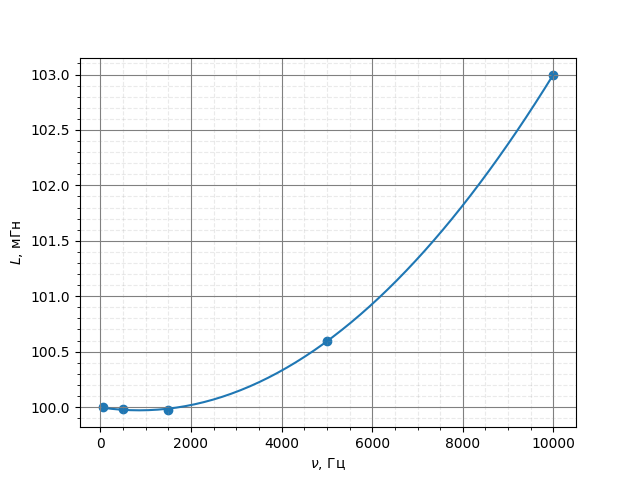
\includegraphics[scale=0.8]{индуктивность.png}
    \caption{Индуктивность в зависимости от чпстоты}
\end{figure}



\begin{figure}[H]
    \centering
    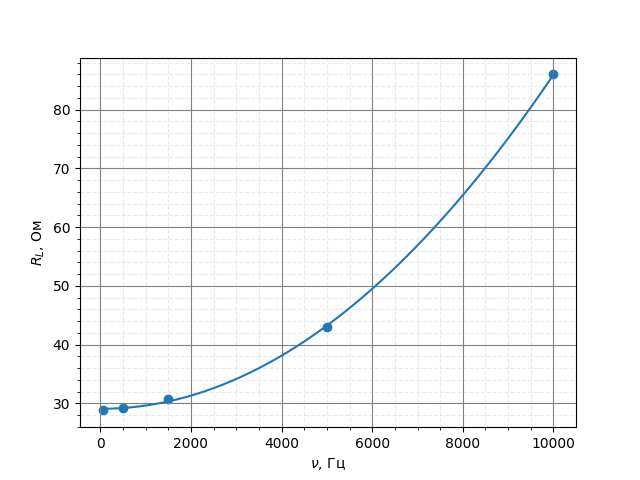
\includegraphics[scale=0.8]{активсопр.png}
    \caption{Активное сопротивление в зависимости от чпстоты}
\end{figure}

\subsection{Измерение периодов свободных колебаний}

L = 100 мГн


\begin{table}[H]
    \centering
    \begin{tabular}{|c|c|c|c|c|c|c|c|c|c|}
    \hline
        C, нФ & 1.0 & 2.0 & 3.0 & 4.0 & 5.0 & 6.0 & 7.0 & 8.0 & 9.0 \\
    \hline
    $\nu$, кГц & 10.87 & 9.04 & 7.8 & 7.04 & 6.44 & 5.94 & 5.58 & 5.25 & 5.02 \\
    \hline
    \end{tabular}
    \caption{Частота свободных колебаний при разной ёмкости}
\end{table}

Экспериментальное значение периода свободных колебаний:
\[T_{\text{эксп}} = \frac{1}{\nu}\]

Теоретическое значение периода свободных колебаний:
\[T_{\text{теор}} = 2\pi \sqrt{LC}\]


\begin{figure}[H]
    \centering
    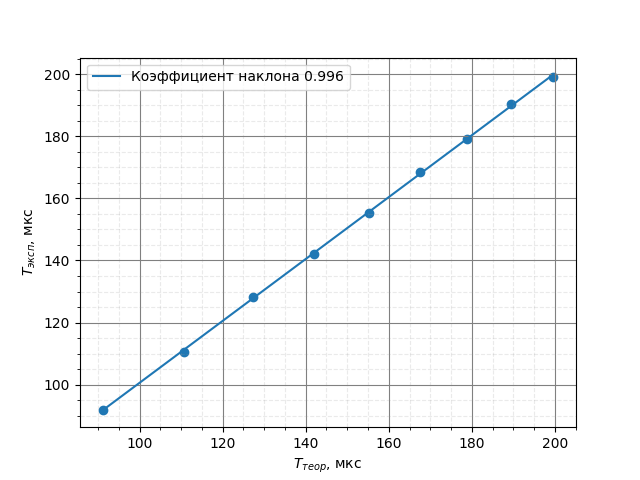
\includegraphics[scale=0.8]{периоды.png}
    \caption{Зависимость $T_{\text{эксп}} = f(T_{\text{теор}})$}
\end{figure}

\[\sigma_{k} = \frac{1}{\sqrt{n}} \sqrt{\frac{<T_{\text{эксп}}^2>-<T_{\text{эксп}}>^2}{<T_{\text{теор}}>-<T_{\text{теор}}>^2}} = 0.05,\]
где k -- коффициент наклона прямой.

\subsection{Критическое сопротивление и декремент затухания}

Примем L = 100 мГн и рассчитаем ёмкость $C^*$, при которой собственшая частота колебаний $\nu_0=1 /(2 \pi \sqrt{L C})$ составляет 6.5 кГц. Для выбраншых $L$ и $C^*$ рассчитаем критическое сопротивление контура $R_{\text{кр}}$ по формуле $R_{\text{кр}}=2 \sqrt{L / C^*}$.

\[C^* = 1.1 \text{ нФ}\]
\[R_{\text{кр}} = 8.2 \text{ кОм}\]

Сопротивление, при котором колебательный режим переходит в апериодический -- 2.9 кОм.

Проведём измерения амплитуд и расчёт декрементов затухзания по формуле (1) для сопротивлений в диапазоне $(0.05-0.25)\cdot R_{\text{кр}}$.

\begin{table}[H]
    \centering
    \begin{tabular}{|c|c|c|c|c|c|c|}
    \hline
         R, Ом & 420 & 574 & 820 & 1230 & 1640 & 2050 \\
         \hline
         $R_{\Sigma}$, Ом & 463 & 617 & 863 & 1273 & 1683 & 2093 \\
         \hline
         $\theta$ & 0.51 & 0.55 & 0.74 & 1.17 & 1.49 & 1.82 \\
         \hline
    \end{tabular}
    \caption{Декременты затухания}
\end{table}


\begin{figure}[H]
    \centering
    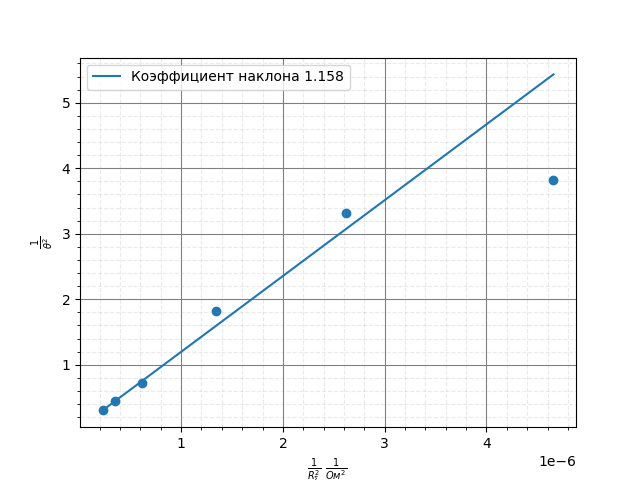
\includegraphics[scale =0.8]{декременты.png}
    \caption{Зависимость $\frac{1}{\theta^2} = f(\frac{1}{R_{\Sigma}^2})$}
\end{figure}

Прямая на графике проведена по первым трём точкам. Приняв обозначения $1 / \Theta^2=Y, 1 /\left(R_{\Sigma}^2\right)=X$, можно показать, что $R_{\mathrm{кр}}=2 \pi \sqrt{\Delta Y / \Delta X}$. Тогда 

\[R_{\text{кр}} = (6761 \pm 26) \text{ Ом}\]

Рассчитаем теоретическое значение $R_{\text {кр }}=2 \sqrt{L / C}$

\[R_{\text{кр}}^{\text{теор}} = 8.2 \text{ кОм}\]

Зафиксируем $R_1 = 420$ Ом и $R_2 = 1640$ Ом.

Рассчитаем добротность контура $Q=\pi / \Theta$ для выбранных значений $R_1$ и $R_2$ по картине затухающих колебаний.
\[Q_1 = 6.1\]
\[Q_2 = 2.1\]

Теоретическое значение добротности по формуле

\[Q = \frac{1}{R_{\Sigma}} \cdot \sqrt{\frac{L}{C}}\]

\[Q_1 = 8.8\]
\[Q_2 = 2.4\]





















\subsection{Свободные колебания на фазовой плоскости}

\begin{table}[H]
    \centering
    \begin{tabular}{|c|c|c|c|c|c|c|}
    \hline
         R, Ом & 420 & 574 & 820 & 1230 & 1640 & 2050 \\
         \hline
         $\theta$ & 0.39 & 0.52 & 0.95 & 1.1 & 2.43 & 2.44 \\
         \hline
    \end{tabular}
    \caption{Декременты затухания}
\end{table}

\[Q_1 = 8.1\]
\[Q_2 = 1.3\]















\subsection{Исследование резонансных кривых}


\begin{table}[H]
    \centering
    \begin{tabular}{|c|c||c|c|}
    \hline
    \multicolumn{2}{|c||}{420 Ом} & \multicolumn{2}{c|}{1640 Ом}  \\
    \hline
    U, В & $\nu$, Гц & U, В & $\nu$, Гц \\
    \hline
         3.2  &  5310  &  0.96  &  4200 \\
\hline
3.6  &  5376  &  1.02  &  4300 \\
\hline
4.0  &  5442  &  1.18  &  4500 \\
\hline
4.4  &  5508  &  1.26  &  4600 \\
\hline
5.0  &  5574  &  1.36  &  4700 \\
\hline
5.4  &  5640  &  1.48  &  4800 \\
\hline
6.1  &  5706  &  1.64  &  5000 \\
\hline
6.8  &  5772  &  1.72  &  5100 \\
\hline
7.4  &  5838  &  1.84  &  5200 \\
\hline
7.7  &  5904  &  2.21  &  5500 \\
\hline
8.0  &  5970  &  2.5  &  6100 \\
\hline
7.6  &  6085  &  2.1  &  7360 \\
\hline
6.9  &  6200  &  1.72  &  8630 \\
\hline
6.2  &  6315  &  1.52  &  9890 \\
\hline
5.3  &  6430  &  1.24  &  13690 \\
\hline
4.8  &  6545  &  1.1  &  18750 \\
\hline
4.2  &  6660  &  1.08  &  21280 \\
\hline
3.9  &  6775  &  1.08  &  23810 \\
\hline
3.6  &  6890  &  1.06  &  26340 \\
\hline
3.4  &  7005  &  1.04  &  28870 \\
\hline
3.2  &  7120  &  1.0  &  31400 \\
\hline 
    \end{tabular}
    \caption{Амплитудно-частотная характреистика}
\end{table}






\begin{figure}[H]
    \centering
    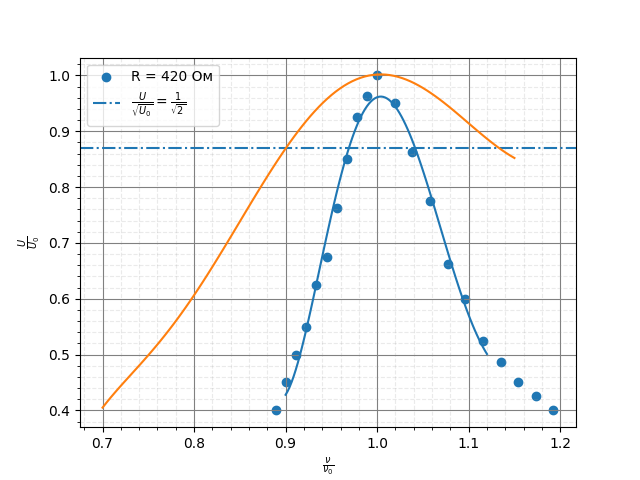
\includegraphics[scale = 0.8]{ачх.png}
    \caption{АЧХ}
\end{figure}

Определим добротности по формуле
\[Q = \frac{\omega_0}{2\Delta \Omega}\]
\[Q_1 = 7.0\]
\[Q_2 = 2.1\]



\begin{table}[]
    \centering
    \begin{tabular}{|c|c||c|c|}
    \hline
    \multicolumn{2}{|c||}{420 Ом} & \multicolumn{2}{c|}{1640 Ом}  \\
    \hline
    U, В & $\nu$, Гц & U, В & $\nu$, Гц \\
    \hline
         68.4  &  6407  &  130  &  3161 \\
\hline
67.2  &  6440  &  116  &  3572 \\
\hline
65.6  &  6473  &  104  &  3983 \\
\hline
64  &  6506  &  93.6  &  4394 \\
\hline
61.6  &  6539  &  84.4  &  4805 \\
\hline
56.4  &  6605  &  74.4  &  5216 \\
\hline
53.6  &  6638  &  65  &  5627 \\
\hline
49.2  &  6671  &  55.8  &  6038 \\
\hline
44.4  &  6704  &  43.2  &  6449 \\
\hline
40  &  6737  &  28  &  6860 \\
\hline
30  &  6803  &  17.2  &  7271 \\
\hline
24  &  6836  &  10.6  &  7680 \\
\hline
19.6  &  6869  &  7.6  &  8090 \\
\hline
17.2  &  6902  &  5.4  &  8504 \\
\hline
14.4  &  6935  &  3.4  &  8920 \\
\hline
12.8  &  6968  &  2.8  &  9330 \\
\hline
11.6  &  7001  &  2.4  &  9740 \\
\hline
10  &  7034  &  1.6  &  10150 \\
\hline
8.8  &  7067  &  1.8  &  10559 \\
\hline
    \end{tabular}
    \caption{Фазочастотная характеристика}
\end{table}





\begin{figure}[H]
    \centering
    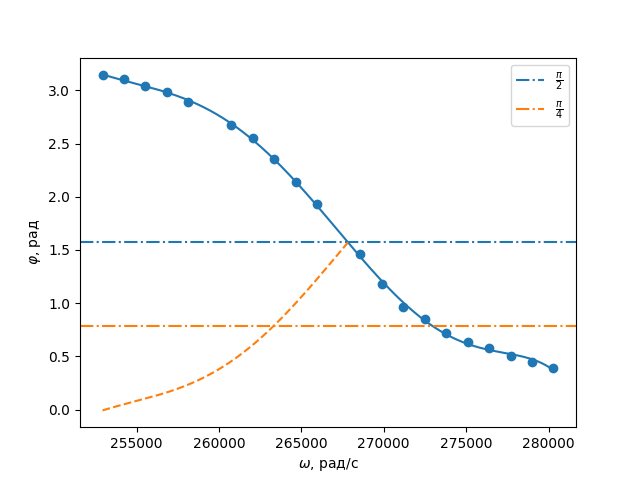
\includegraphics[scale=0.8]{фчх1.png}
    \caption{ФЧХ при $R_1$ Ом}
    \label{fig:enter-label}
\end{figure}



\begin{figure}[H]
    \centering
    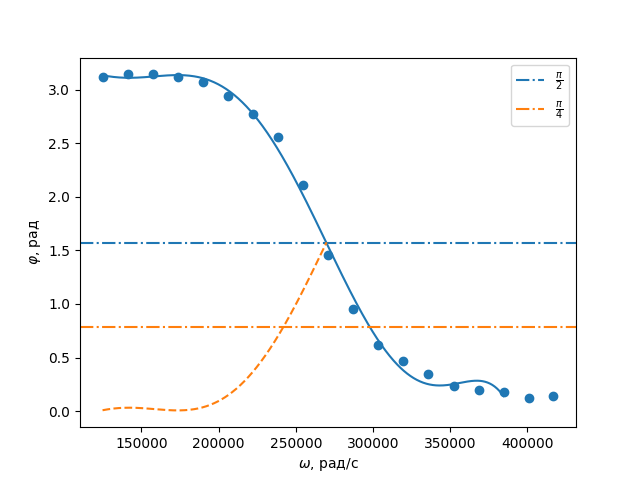
\includegraphics[scale=0.8]{фчх2.png}
    \caption{ФЧХ при $R_2$ Ом}
    \label{fig:enter-label}
\end{figure}

Добротность по ФЧХ
\[Q = \frac{\omega}{\Delta \omega}\]
\[Q_1 = 5.5\]
\[Q_2 = 2.4\]


Определим добротности по затуханию и нарастанию колебаний.
При нарастании
\[\Theta=\frac{1}{n} \ln \frac{U_0-U_k}{U_0-U_{k+n}}\]
\[Q = \frac{\pi}{\theta}\]
\[Q_1 = 7.3\]
\[Q_2 = 2.4\]

При затухании $\theta$ вычисляется по формуле (1)
\[Q = \frac{\pi}{\theta}\]
\[Q_1 = 8.1\]
\[Q_2 = 2.6\]









\begin{table}[H]
\centering
\begin{tabular}{|c|c|c|c|c|c|c|c|}
\hline
$R,$ Ом & $f(L, C, R)$ & $f(\theta)$ & Спираль & АЧХ & ФЧХ & Нарастание & Затухание \\ \hline
420 & 8.8 & 6.1 & 8.1 & 7.0 & 5.5 & 7.3 & 8.1 \\
\hline
1640 & 2.4 & 2.1 & 1.3 & 2.1 & 2.4 & 2.4 & 2.6 \\
\hline
\end{tabular}
\caption{Итоговая таблица с результатами измерения добротности}
\label{tab:final_table}
\end{table}
\section{Вывод}

Экспериментальные и теоретические значения очень хорошо совпадают с учётом поправки на индуктивность контура.

Аппроксимация резонансных кривых производилась полиномиальной функцией высокого порядка методом наименьших квадратов. На самом деле функции АЧХ и ФЧХ не являются полиномами, отсюда возникает достаточно большая погрешность расчёта добротности.




\end{document}


